\documentclass{article}
\usepackage{latexsym}
\usepackage{amsmath}
\usepackage[a4paper]{geometry}
\usepackage{fullpage}
\usepackage{hyperref}
\usepackage{booktabs}
\usepackage{graphicx}
\usepackage{tikz}
\usepackage{xcolor}
\usepackage[export]{adjustbox}
\usepackage{comment}
\usepackage{subcaption}
\usepackage[style=iso]{datetime2}
\usepackage{cleveref}
%\usetikzlibrary{calc}
\usetikzlibrary{arrows,positioning} 
\tikzset{
    %Define style for course boxes
    courseboxv/.style={
           rectangle,
           draw=blue!50!black, very thick,
           fill=blue!10,
           minimum height=8cm,
           minimum width=4cm,
           text width=3.9cm,
           text centered,
           font=\bfseries\sffamily},
    courseboxh/.style={
           courseboxv,
           minimum height=4cm,
           minimum width=8cm,
           text width=7.9cm},
    courseboxhh/.style={
           courseboxh,
           minimum height=4cm,
           minimum width=16cm,
           text width=15.9cm}
}
\def\frameseparation{1.5cm}
\def\scalingfactor{.8}

\newcommand{\secref}[1]{Section~\ref{sec:#1}}
\newcommand{\secreff}[2]{Sections \ref{sec:#1} and \ref{sec:#2}}
\newcommand{\eqnref}[1]{Equation~\eqref{eq:#1}}
\newcommand{\eqnreff}[2]{Equations \eqref{eq:#1} and \eqref{eq:#2}}
\newcommand{\eqnrefff}[3]{Equations \eqref{eq:#1}, \eqref{eq:#2} and \eqref{eq:#3}}
\newcommand{\figref}[1]{Figure \ref{fig:#1}} 
\newcommand{\figreff}[2]{Figures \ref{fig:#1} and \ref{fig:#2}}
\newcommand{\figrefff}[3]{Figures \ref{fig:#1}, \ref{fig:#2} and \ref{fig:#3}}
\newcommand{\tabref}[1]{Table~\ref{tab:#1}}
\newcommand{\tabreff}[2]{Tables~\ref{tab:#1} and \ref{tab:#2}}
\newcommand{\tabrefff}[3]{Tables~\ref{tab:#1}, \ref{tab:#2} and \ref{tab:#3}}

\def\year{2024--2025}
\title{EITA65 Design of Systems for Digital Transformation\\\year}
%\title{EITA65 Digitalisering -- realisering och systemdesign med användarperspektiv\\\year}
\author{\huge Route Planning\\Drone Project -- Part 3}
%\\Version \DTMnow}
%\date{}

\begin{document}
\newgeometry{left=2.5cm,right=2.5cm,bottom=1.5cm}% for placing course schematic lower on first page
\clearpage\maketitle
\thispagestyle{empty}% to remove page numbering on first page

\begin{itemize}
\item 
\includegraphics[width=3mm]{person.png}
\includegraphics[width=3mm]{person.png} This project will be done in pairs, but you will work \textit{together} in groups of 3 or 4.
\item You will not get detailed step-by-step instructions. Figuring out how to reach the goal is part of the project. (being a collaborative doer)
\item The results of this project part will be used in the next, so document your work.
\end{itemize}

\vspace{.1cm}
\begin{center}
\begin{tabular}{l}
\toprule[1.5pt]
\parbox{0.8\linewidth}{
\vspace{.2cm}{\Large Learning goals:}
\begin{itemize}
\item Becoming familiar with web server development
  \begin{itemize}
  \item Understanding interactions with multiple servers.
  \item Learn to interact with a Redis database. 
  \end{itemize}
\item Take a bite of \texttt{geopy}.
\item Write a simple route planning algorithm on your own.
\item Practicing collaboration skills.
\end{itemize}}\\
\bottomrule[1.5pt]
\end{tabular}
\end{center}
\vfill
\begin{center}
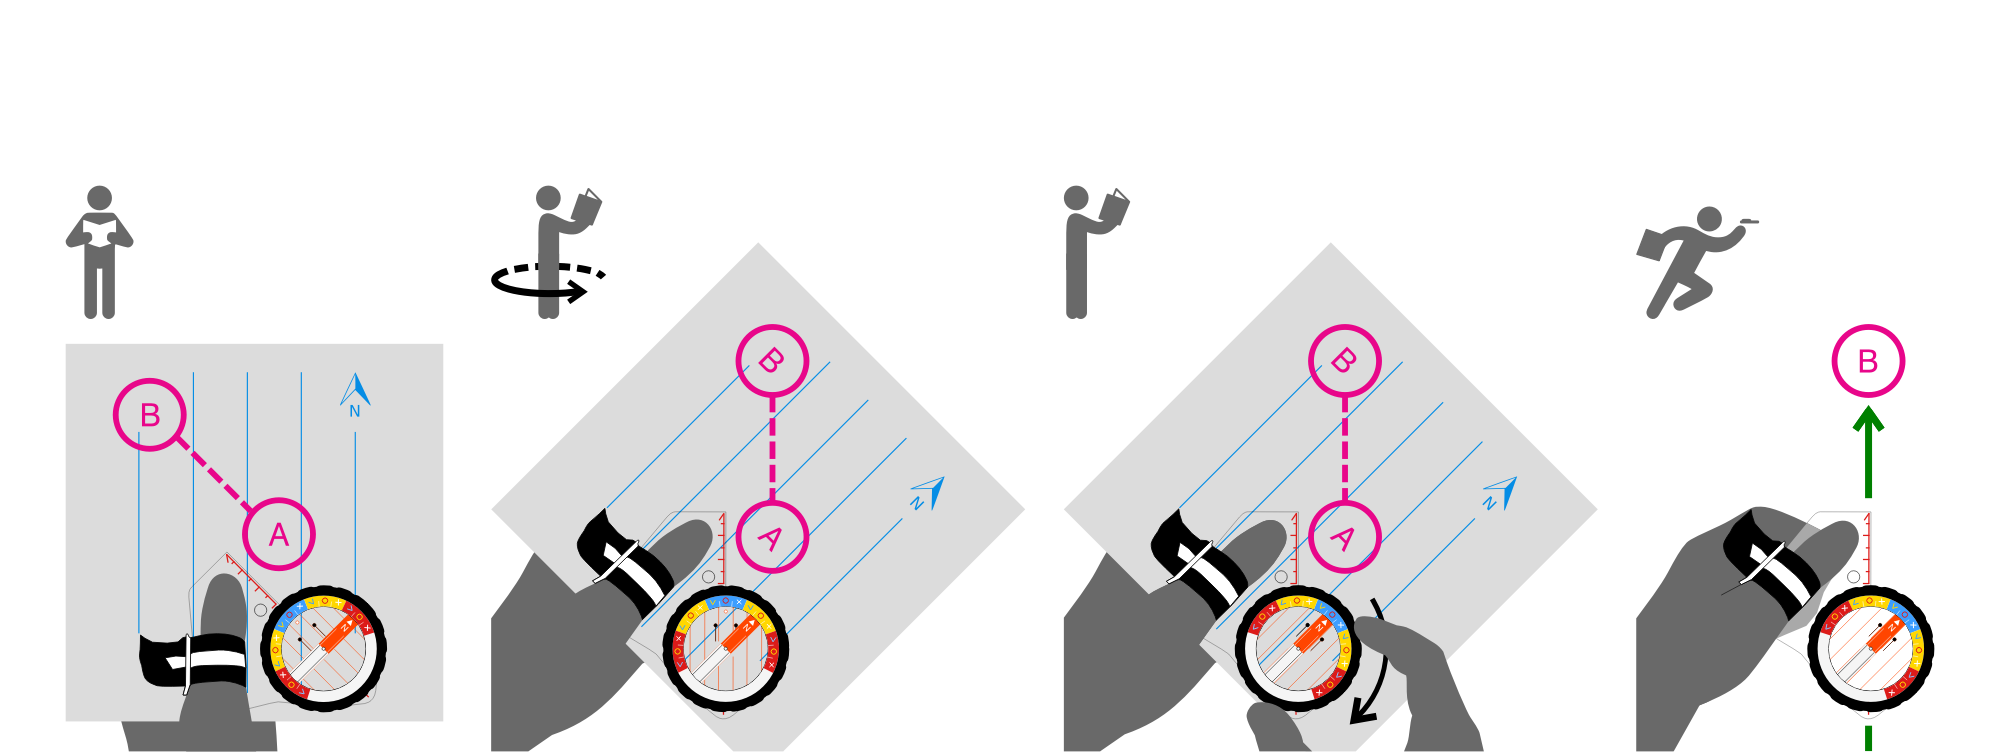
\includegraphics[width=120mm]{orienteering.png}
\end{center}
\vspace{2cm}

\begin{comment}
\begin{center}
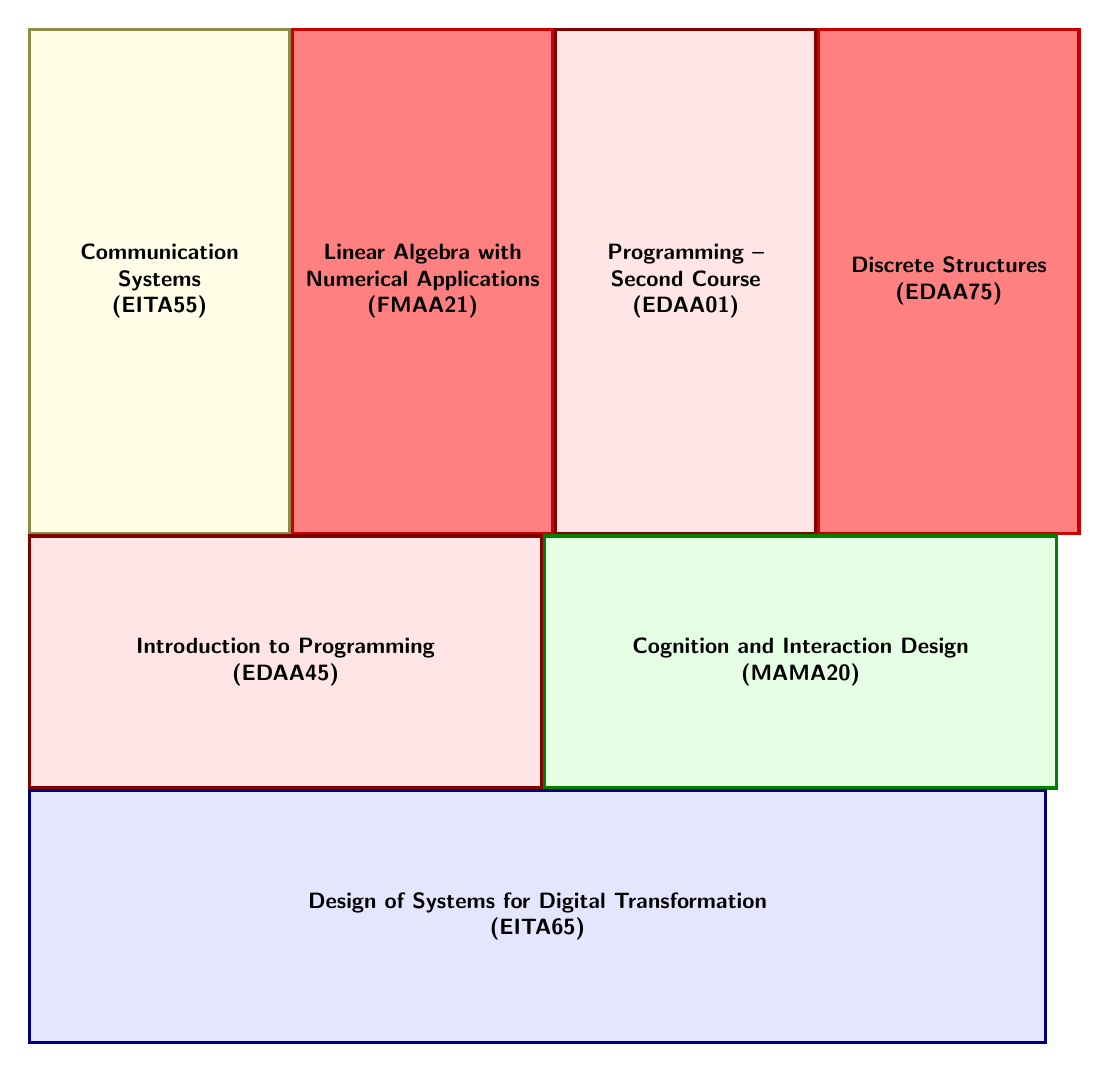
\begin{tikzpicture}[>=latex, node distance=0cm,scale=\scalingfactor,every node/.style={scale=\scalingfactor}]
\node[courseboxv, draw=yellow!50!black, fill=yellow!10] (EITA55) {Communication Systems\\(EITA55)};
\node[courseboxv, draw=red!80!black, fill=red!50, anchor=west] (FMAA21) at (EITA55.east){Linear Algebra with Numerical Applications\\(FMAA21)};
\node[courseboxv, draw=red!50!black, fill=red!10, anchor=west] (EDAA01) at (FMAA21.east){Programming -- Second Course\\(EDAA01)};
\node[courseboxv, draw=red!80!black, fill=red!50, anchor=west] (EDAA75) at (EDAA01.east){Discrete Structures\\(EDAA75)};
%\node[courseboxh, preaction={clip, postaction={fill=red!10, draw=red!50!black, line width=2mm}}, anchor=north west] (EDAA45) at (EITA55.south west){Introduction to Programming\\(EDAA45)};
\node[courseboxh, draw=red!50!black, fill=red!10, anchor=north west] (EDAA45) at (EITA55.south west){Introduction to Programming\\(EDAA45)};
%\node[courseboxh, draw=green!50!black, fill=green!10, anchor=west] (MAMA20) at (EDAA45.east){Cognition and Interaction Design\\(MAMA20)};
\node[courseboxh, draw=green!50!black, fill=green!10, right=of EDAA45] (MAMA20) {Cognition and Interaction Design\\(MAMA20)};
\node[courseboxhh, anchor=north west] (EITA65) at (EDAA45.south west){Design of Systems for Digital Transformation\\(EITA65)};
%\node[anchor=south east, inner sep=2pt, font=\bfseries\sffamily\scriptsize] at (EDA625.south east) {Helsingborg};
%\path[->,draw=black,dotted,thick] (EIT060.east) -- (EITF05.west);
%\path[->,draw=black,dotted,thick] (EIT060.south) -- (EITN50.north);
%\path[->,draw=black,dotted,thick] (EITF05.south) -- (EITN41.north);
%\draw[draw=blue!50!black, very thick] ($(EIT060.north west)+(-\frameseparation,\frameseparation)$) rectangle ($(EDA625.south east)+(\frameseparation,-\frameseparation)$);
\end{tikzpicture}
\end{center}
\end{comment}

\restoregeometry
\newpage


\section{Introduction}
In this project part you will need to write a simple route planner for your drone in the simulation. You will get the coordinates of any two addresses in Lund, and plan a path for your drone to reach the destination. 

You will write your own code based on {\color{blue}\href{https://github.com/HaoruiPeng/InfoCom-LP2-Lab3}{this GitHub repository}}. This is very similar to what you were working on in the two previous parts, Drone simulation on Raspberry Pi and Microservices, but you no longer need your joystick or keyboard on Raspberry Pi to control your drone. Instead, you write your own code so that your drone
\begin{itemize}
    \item autonomously plans a path to move along,
    \item sends updates of its real-time location to the Redis database along the way.
\end{itemize}
As for the previous labs, you are recommended to fork and clone from your own repository.

In this lab, you have three Flask servers, and you need to have all of them running to have a functional application. Before you run the code by following \verb!README.md!, make sure you changed the Redis server URL on all server scripts, so that all the servers can read and write drone location data from the database.

Since you no longer need the joystick on Raspberry pi, you can run this code on any of the devices you have; Raspberry Pi, your own computer or a lab computer. Your device just needs to have an Internet connection.\vspace{0.3cm}

\noindent{\bf Note: }\parbox[t]{14cm}{{You will get some questions marked in red in this instruction. You need to write down the answers and show to the TAs when you present your work.}}\vspace{0.2cm}

\section{Application Architecture}

In this application, you have three Flask servers running. When you fill in your own Redis URL in all three server scripts, you should be able to run the application with no error. When you have every server up and running, open the website hosted by \verb!build.py!, you will see the same map as you saw in previous labs, but with a new form.

The form asks you to write two addresses, [From address] and [To address]. These are two addresses of your path that you want your drone to fly along. You can input any real addresses in Lund, and search for them. The two addresses will be submitted to the server \verb!route_planner.py!, which retrieves their OSM coordinates in (longitude, latitude).

\vspace{0.5cm}
\noindent{\bf Question 1: }\parbox[t]{13cm}{\textcolor{red}{Take a look at \texttt{route\_planner.py} and \texttt{index.html}. What is the URL of the new route planner server?}} \vspace{0.5cm}

The new route planner server takes the input addresses, and sends it to OpenStreetMap using \verb!geopy.geocoders.Nominatim!, which is a Python API that provides the commutation to OpenMapStreet to get the geographical information of a real address. In this application we are only interested in the longitude and latitude values of an address. When you submit the two addresses, you will have a window pop up, and it tells you whether the server can find the two addresses or not. If it could not, then you need to write a new address.

The route planner will invoke the \verb!/pi/pi_controller.py! script when it finds the two input addresses correctly.
Thus in this project part, you do not need to run this script separately in another terminal. Contrary to what you did in the previous project parts, the \verb!/pi/pi_controller.py! in this lab should send its current location in (longitude, latitude) to the database server (instead of the direction of movement). Therefore, in \verb!database.py!, the script only takes the values sent from \verb!/pi/pi_controller.py!, and stores them in Redis, without any further processing.

\vspace{0.5cm}
\noindent{\bf Question 2: }\parbox[t]{13cm}{\textcolor{red}{\Cref{fig:drone} shows the application architecture we used in instruction Part 2. Please add a new block to this figure, representing the \texttt{route\_planner} server, and add arrows to the other components it communicates with, and explain which messages are exchanged along the newly added message paths (the arrows). } } \vspace{0.5cm}

\begin{figure}[h!]
    \centering
    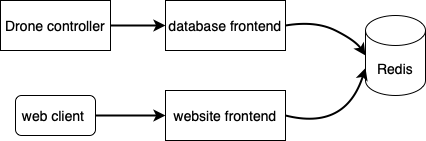
\includegraphics[width=80mm]{drone-system-architecture.drawio.png}
    \caption{Application architecture of a drone simulation system.}
    \label{fig:drone}
\end{figure}

\section{Write a route planner}

When the route planner invokes \verb!pi_controller.py!, three pairs of coordinates are passed to the controller. The three pairs of coordinates are printed in the terminal that runs the route planner.

\vspace{0.5cm}
\noindent{\bf Question 3: }\parbox[t]{13cm}{\textcolor{red}{Note down the three pairs of coordinates, and explain which location each coordinate pair represents, and how the route planner got the values.} } \vspace{0.5cm}

You need to use the three coordinate pairs to write your own function (now called \verb!your_function()!) in \verb!pi_controller.py!. The function needs to plan the path and move your drone. In the provided code the functionality \textit{is not completed}, so you will not see your drone moving, and it only updates the database with an initial location. You need to complete the code by following the comments in the code. The provided function is a guiding example, and it indicates what should be returned and what should be sent to the database server. You can structure your code as you find best, writing one or multiple functions. You also need to update the \verb!run()!-function so that it matches what you are doing in your route planning function.

The functionalities the script should have are:
\begin{itemize}
    \item Three coordinate pairs are passed to the \texttt{run()} function. The three coordinate pairs represent your drone's current location, the [from address] and [to address] you wrote in the web browser. You need use these coordinates to plan a path, and write a function to move your drone along this path. Your drone should first move from its current location to the [from address], and then from [from address] to the [to address].
    \item The condition of the \verb!while! loop is \verb!True!, and in every iteration of the loop, it sends your drone's new location to the server. You need to change the halt condition so that the loop stops when your drone reaches the [to address].
    \item Instead of "jumping" from one place to another, your drone should appear to move continuously along the path. Therefore, while moving, your drone needs to keep updating its location often enough. (Consider the \verb!moveDrone()! function we used in the previous instruction parts.)
\end{itemize}

%\section{Hint for MAC OS}
%\label{sec:mac}
%If you run the web server on MAC OS, you may get problems with \verb!pip3!. MAC has Python3 installed by default in the system, but not \verb!pip3!. There are several ways to install \verb!pip3! if you use the search phrase \textit{How to install pip3 on MAC OS}. The easiest one you find may be \verb!brew install python3!. The command \verb!brew! is the most popular package manager on MAC OS (like \verb!apt! in Debian), but when you install with \verb!brew!, you install the whole python3 again in your system, but in a different path. This path is not in your default system PATH, so your computer will not understand that you wants to use the newly installed python3. Therefore, you need to add the new path to your system PATH in \verb!~/.bash\_profile! or \verb!~/.zshrc!, then \verb!source! the changed file and you should be able to use the newly installed \verb!python3! and \verb!pip3!.

% {\bf Hint 1: }\parbox[t]{14cm}{Check for updates to this document. Instructions may have been clarified in a more recent version. You can find the version number of the document on the very first page. The version number is the compile-date of the document in ISO-format~\cite{iso-date-time}.}\\
% {\bf Hint 2: }\parbox[t]{14cm}{To avoid rewriting many commands, you can use the keys \texttt{arrow up} and \texttt{arrow down} to go back and forth between the commands that you just wrote.}\\
% {\bf Hint 3: }\parbox[t]{14cm}{To paste commands into the terminal you can use \texttt{Ctrl + Shift + V}}\\
% {\bf Hint 4: }\parbox[t]{14cm}{tab in instructions}\\
% {\bf Hint 5: }\parbox[t]{14cm}{To avoid rewriting many commands, it can be a good idea to write all steps in a batch-file or shell script. Then you can also reuse the batch file for the second project.}

\section{Hints on writing your route planner}

The route planner can be written in several way, utilizing different strategies. Here we outline two different approaches, any of which you might find useful.

\subsection{Method 1}

The idea here is to move a single step in the direction of the target each time \texttt{your\_function()} is called. We need to keep track of the current drone position and the current target.

Begin by setting the current target to the from position. In \texttt{your\_function()}, check if you are very close to the target. If so, return the position of the target. Else, check if you are more than one step away from the target along the X axis and, if so, move one step along the X axis towards the target. Do the same for the Y axis. When you reach the target, and the target is the from position, change the target to the to position.

If you solve the problem like this the drone will only move in the cardinal (north, east, south, west), and intercardinal (northeast, southeast, southwest, northwest) directions. If you like, you can instead calculate and return the position one step away from the current position directly in the direction of the target using your trigonometry skills from high school.


\subsection{Method 2}

This method makes use of the observation that the task of moving from one point to another point via a third point can be divided into two easier tasks. The entire contents of the \texttt{run()} method could be replaced by two calls to a function performing a single trip between two positions -- first from the current position to the from position and then from the from position to the to position:

\vspace{2mm}

\texttt{travel(current,from)}


\texttt{travel(from,to)}

\vspace{2mm}

In the \texttt{travel()} function you can then use a simple for loop to visit a suitable number of positions along the line from the starting point to the end point. You should be able to use your math knowledge about geometry and similar triangles from high school to calculate the positions of the points along the line. Each time you have calculated the next position you need to send the new position to the database. At the end of the given \texttt{run()} function you can see how to do this (check out the code starting with ''\texttt{with requests.Session() as session:}'').




\vspace{1cm}
\begin{center}
\huge Good luck!
\end{center}

% \begin{thebibliography}{10}
% \bibliographystyle{plain}
% 
% \bibitem{MD} Google's microservice demo, \url{https://github.com/GoogleCloudPlatform/microservices-demo}, last accessed on 2021-11-12.

% \bibitem{OSM} OpenStreetMap, \url{https://www.openstreetmap.org/#map=14/55.7059/13.2005}, last accessed on 2021-11-08.

% \bibitem{deco} Python decorator, \url{https://python-3-patterns-idioms-test.readthedocs.io/en/latest/PythonDecorators.html}, last accessed on 2021-11-08.


% \end{thebibliography}

\end{document}
